\section{Executive Summary}
\setlength{\parskip}{0pt plus 4pt}

\subsection{Outline requirements}

\begin{itemize}
   \item Construct an indoor environment with a human model in it in Gazebo Classic for testing autonomous navigation and face detection funtionality.
   \item Implement autonomous navigation on the robot designed in the last assignment.
   \item Implement face detection on the robot.
   \item Test the robot in different navigation scenarios.
   \item Detect the face of the human model and snapshoot the face.
\end{itemize}


\subsection{Redesigning robot from the assignment 1}

Assignment 1 only requires the design of the structure of a robot. To deploy the navigation framework and the face detection algorithm and simulate on Gazebo Classic, necessary information should be added to the robot description, and parts of the description should be adapted to the requirement of the simulator, the framework and the algorithm.

Three Gazebo-ROS sensoring plugins were added. They are libgazebo\_ros\_gpu\_laser, libgazebo\_ros\_imu\_sensor, and libgazebo\_ros\_camera. The laser plugin and IMU plugin are required by the navigation framework. The camera plugin is essiensial to any computer vision algorithm.

Two control plugins, libgazebo\_ros\_control and libgazebo\_ros\_skid\_steer\_drive were added. The former was used to control manipulator mounted on the robot. The latter functions as a controller of drives, which subscribes a command velocity topic and publishes an odometry topic. These are the two de facto ROS package APIs. The major component of the navigation framework, move\_base, which will be introduced latter, and other packages used in this assignment, depend on these two APIs.


\subsection{Consturcting simulation environment}

\begin{figure}[htbp]
   \centering
   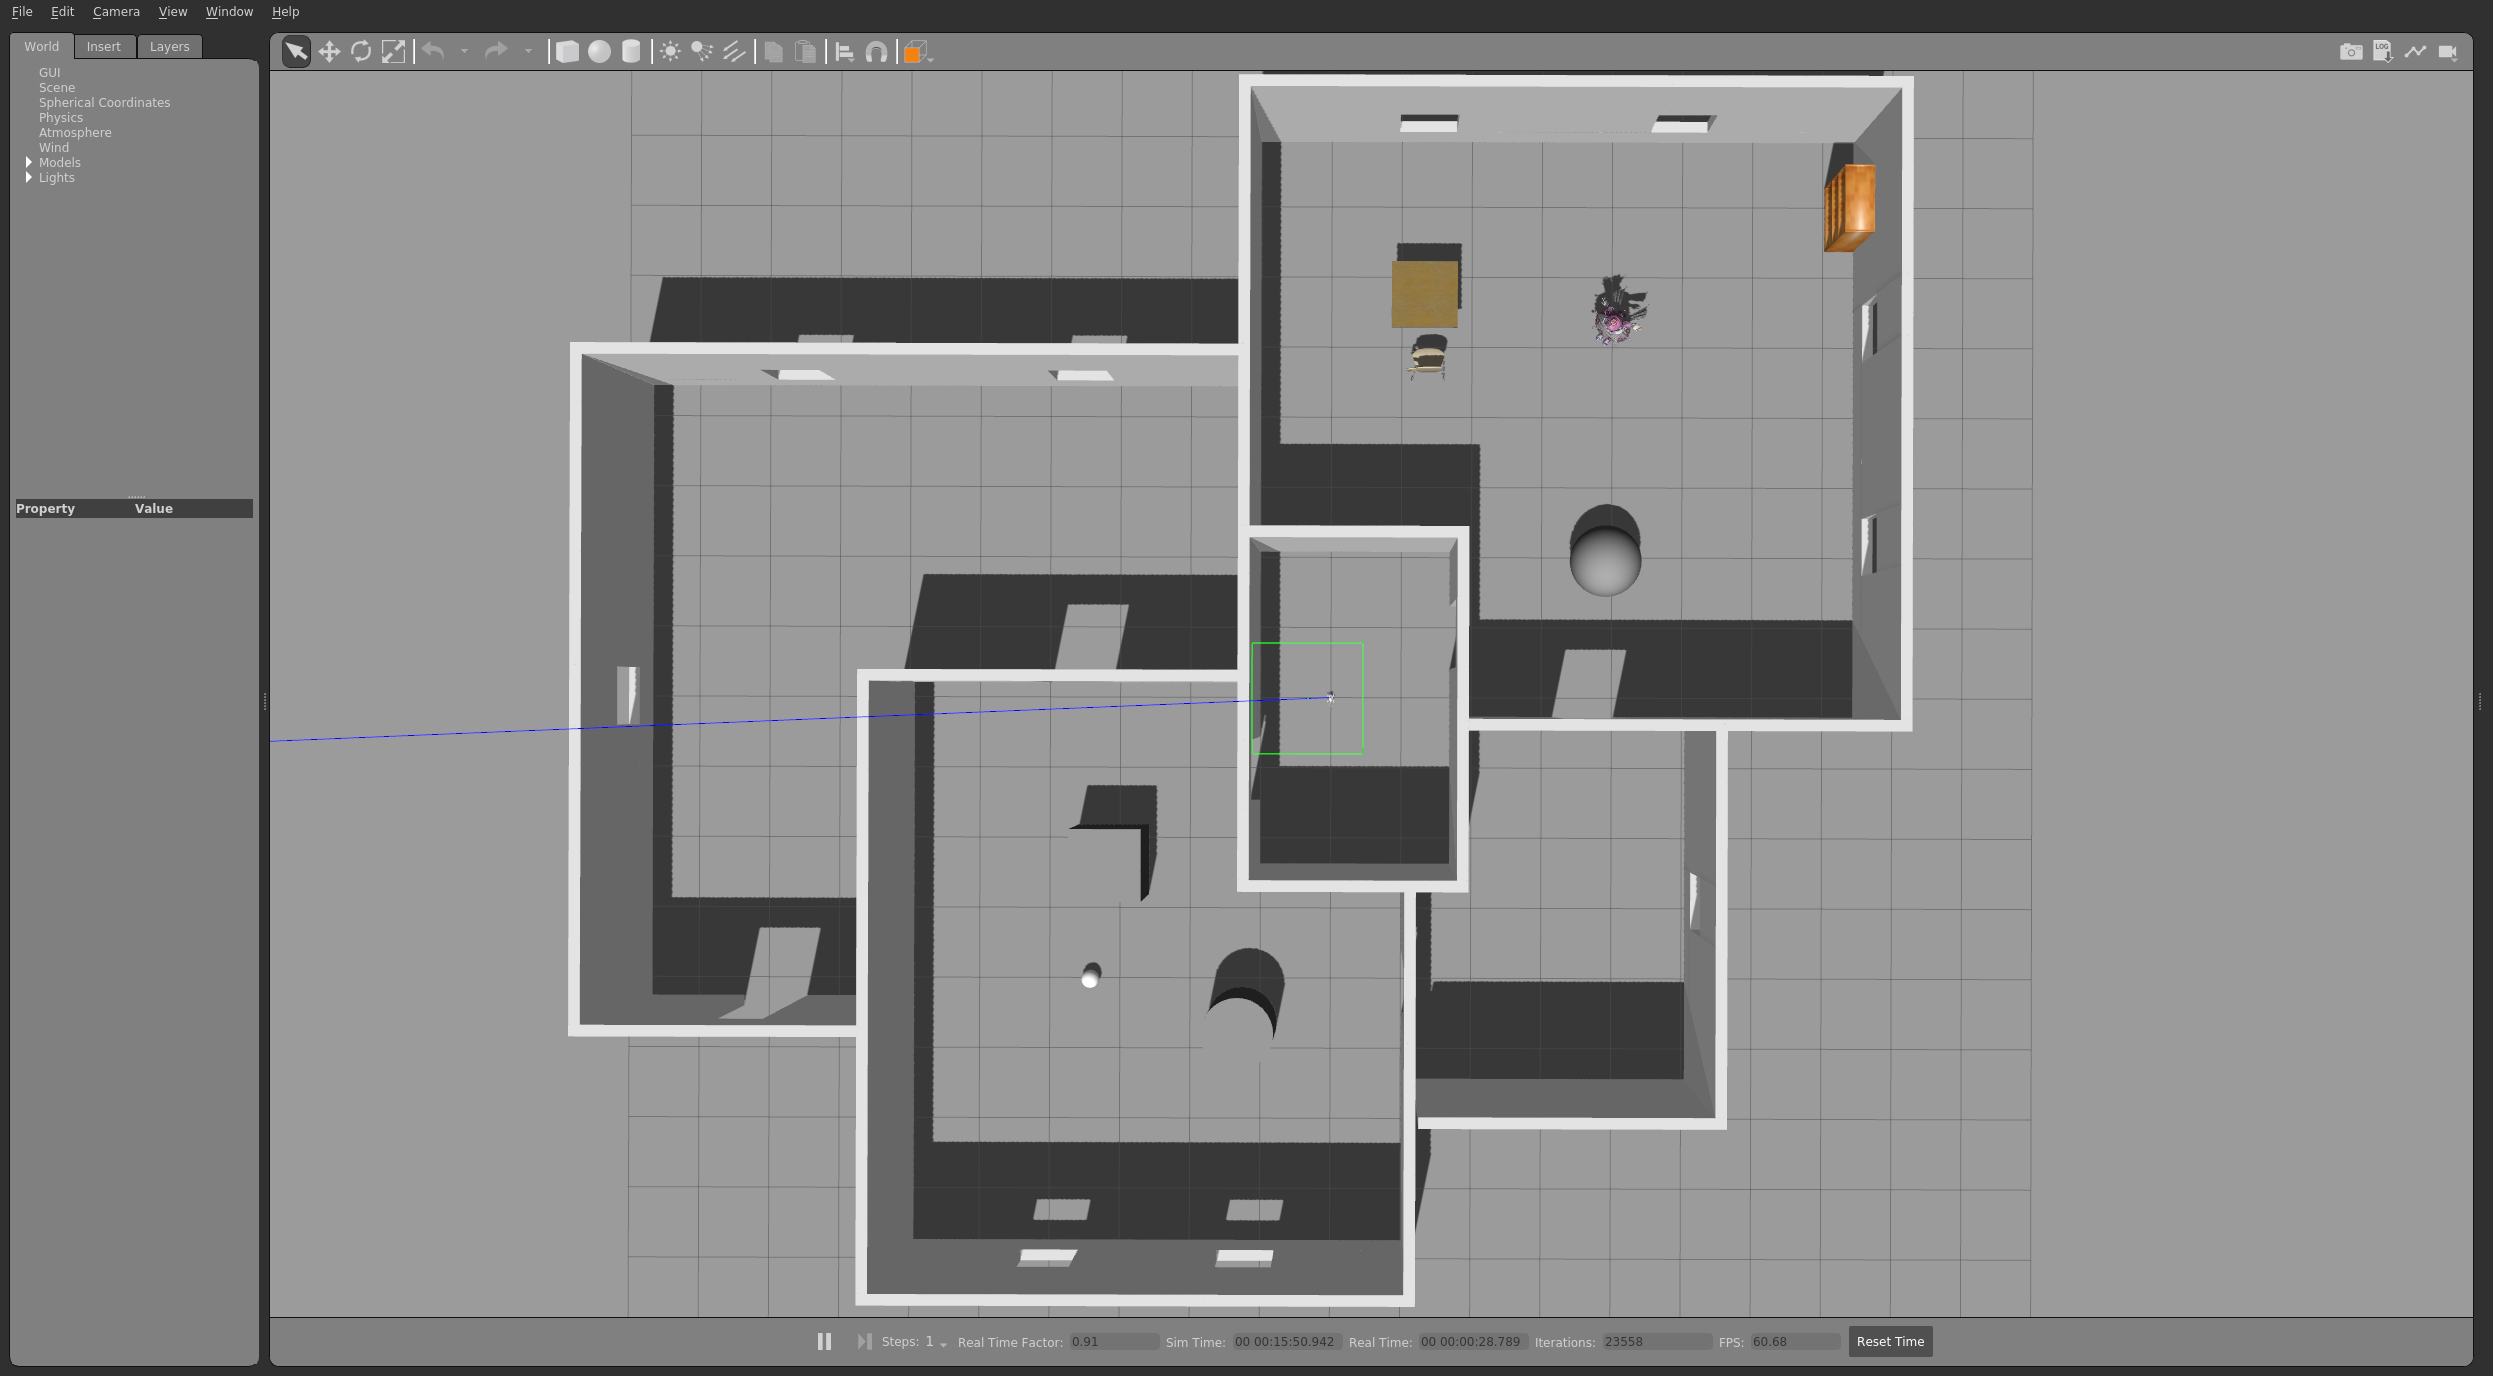
\includegraphics[width=0.5\textwidth]{birdview.png}
   \caption{Aerial view of the simulation environment}
   \label{fig:birdview}
\end{figure}

Figure~\ref{fig:birdview} shows the bird's-eye view of the simulation environment. The human model is placed at the top right of the figure. Several static obstacles scattered throughout the environment.

The layout of the environment, including walls, windows, and doors, were set by the Gazebo Classic built-in building editor. Regular-shaped objects can be directly accessed on the tool bar. The coffee table and bookshelf are recorded in Gazebo databases which can be accessed in the insert tab on the left-side bar of the GUI. Coffee cup-shaped chair and anime character model were downloaded from MikuMikuDance (MMD) file hosting websites and were converted to COLLADA which Gazebo Classic can read by Blender with MMD Tools addon. Exported COLLADA files were imported into Gazebo Classic model editor to further convert the model into Gazebo model format called Simulation Description Format (SDF). After all the objects were prepared, they were inserted into default empty world to produce a world file which describes the indoor environment as shown in Figure~\ref{fig:birdview} in SDF.


\subsection{Navigation after simultaneous localisation and mapping (SLAM)}

Methods provided in the navigation framework are mainly map-based, so a map is required to use the framework for autonomous navigation. A famous issue associated with mapping is abbreviated as SLAM. With the help of ROS slam-gmapping package, mapping is fairly easy to do. As the name suggests, SLAM includes localisation and mapping, so two nodes are required for this task. Adaptive Monte Carlo localisation (AMCL) node and Gmapping node were used in this assignment, plus a keyboard control node for moving robot manually. Instead of AMCL, odometry localisation was also tried and produced similar result.

After the first stage, generated map were saved and then loaded into map server node. The map server node publishes a map topic so that the major component of the navigation framework, move\_base, can access and interpret the map, plan global path and local path, and move the robot towards the navigation goal.

Most of the time was spent on tuning parameters of navigation components. There are dozens of parameters in total, but the official tuning guide is poorly written. Tuning a smooth navigation behaviour is basically a matter of luck. Parameters that have been adjusted in one environment may not be suitable in another. Recovery behaviour was found to be cumbersome, so it was disabled.


\subsection{Face detection}

YOLOv5, an object detection model, was trained on a subset of a face dataset, WIDER FACE, for detecting faces. Few lines of Python code was written to glue the model with the robot and RViz. Figure~\ref{fig:face-detection} demostrates the results visualised in RViz.

\begin{figure}[htbp]
   \centering
   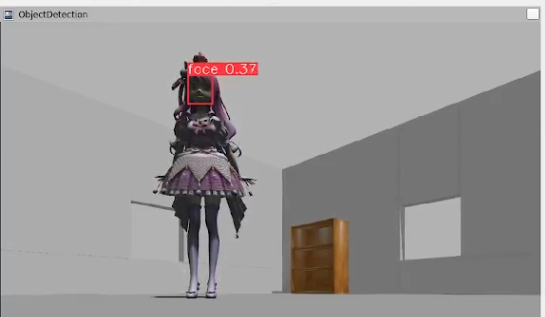
\includegraphics[width=0.5\textwidth]{face-detection.png}
   \caption{Face of the anime character model was detected but with low confidence}
   \label{fig:face-detection}
\end{figure}

The model often failed to detect the face of anime character model. Even when it did, it had a low confidence on the result, as illustrated in the figure. This may be due to the insufficient training data (1.5G data was picked from original 25G dataset) and the fact that there are only real faces in the dataset, while during the test, anime face was the predicting target. Texture of the face appeared dim in Gazebo Classic, which may also be a reason.
